\par\SourceLeaf{265}%
\noindent 1. Ist $d\omega$ ein unendlich kleiner Centriwinkel $ACB$ eines Kreises vom Radius $AC=BC=r$, so ist der zugeh\"orige unendlich kleine Bogen $AB=ds$ proportional $d\omega$, und der Proportionalit\"atsfactor h\"angt nur von $r$ ab. Man hat daher:

\[
\tag*{(A)} ds = f(r)\,d\omega.
\]

\begin{center}\begin{minipage}{\linewidth}\centering
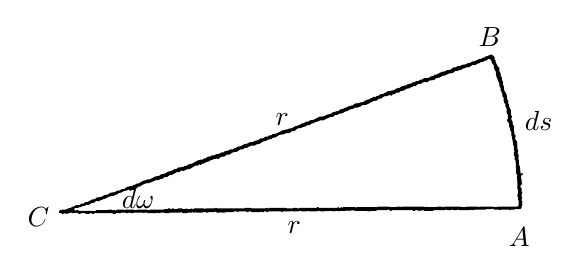
\begin{tikzpicture}[x=0.00765864cm,y=-0.00765864cm]
\fill[even odd rule] (847,257) -- (844,257) -- (843,256) -- (842,245) -- (841,244) -- (840,233) -- (839,232) -- (840,230) -- (840,226) -- (838,223) -- (839,221) -- (839,218) -- (838,217) -- (838,210) -- (837,209) -- (838,206) -- (836,202) -- (834,200) -- (835,194) -- (833,192) -- (833,189) -- (832,188) -- (832,178) -- (830,175) -- (830,171) -- (828,168) -- (828,165) -- (829,163) -- (827,159) -- (827,152) -- (824,146) -- (824,143) -- (823,142) -- (823,138) -- (821,134) -- (820,126) -- (816,119) -- (815,111) -- (814,110) -- (814,105) -- (812,102) -- (812,98) -- (810,94) -- (810,91) -- (808,88) -- (808,82) -- (805,79) -- (802,73) -- (802,70) -- (800,68) -- (800,64) -- (796,60) -- (793,60) -- (787,63) -- (785,63) -- (783,65) -- (781,65) -- (778,67) -- (775,67) -- (767,71) -- (764,71) -- (759,74) -- (756,74) -- (753,76) -- (746,77) -- (743,79) -- (739,79) -- (736,81) -- (732,81) -- (727,85) -- (721,86) -- (717,88) -- (714,88) -- (704,93) -- (701,93) -- (699,95) -- (695,96) -- (692,98) -- (690,98) -- (689,99) -- (683,99) -- (681,101) -- (676,102) -- (674,104) -- (670,104) -- (667,106) -- (664,106) -- (662,108) -- (659,108) -- (658,109) -- (656,109) -- (654,111) -- (651,111) -- (650,112) -- (645,113) -- (643,115) -- (638,116) -- (633,119) -- (622,121) -- (620,123) -- (618,123) -- (616,125) -- (610,126) -- (608,128) -- (604,129) -- (603,130) -- (599,130) -- (597,132) -- (595,132) -- (593,134) -- (588,135) -- (581,139) -- (578,139) -- (577,140) -- (574,140) -- (573,141) -- (569,141) -- (565,144) -- (563,144) -- (562,145) -- (557,146) -- (554,148) -- (552,148) -- (549,150) -- (544,151) -- (542,153) -- (531,156) -- (529,158) -- (521,160) -- (519,162) -- (510,163) -- (500,168) -- (494,169) -- (491,171) -- (488,171) -- (483,174) -- (481,174) -- (476,177) -- (469,179) -- (464,182) -- (458,183) -- (457,184) -- (454,184) -- (453,185) -- (450,185) -- (438,191) -- (432,192) -- (429,194) -- (426,194) -- (424,196) -- (420,196) -- (416,199) -- (412,199) -- (408,202) -- (405,202) -- (399,205) -- (395,205) -- (389,208) -- (386,208) -- (379,212) -- (373,213) -- (371,215) -- (369,215) -- (367,217) -- (362,217) -- (359,219) -- (353,220) -- (351,222) -- (348,222) -- (342,225) -- (339,225) -- (335,227) -- (332,227) -- (328,229) -- (325,229) -- (321,232) -- (319,232) -- (316,234) -- (312,234) -- (311,235) -- (309,235) -- (298,241) -- (295,241) -- (288,245) -- (286,245) -- (285,246) -- (281,246) -- (280,247) -- (276,247) -- (272,250) -- (269,250) -- (264,253) -- (259,254) -- (254,257) -- (246,259) -- (244,261) -- (238,262) -- (228,267) -- (224,267) -- (223,268) -- (218,269) -- (209,274) -- (206,274) -- (204,276) -- (202,276) -- (199,278) -- (195,278) -- (194,279) -- (192,279) -- (188,281) -- (186,283) -- (182,283) -- (179,285) -- (173,286) -- (171,288) -- (163,289) -- (159,292) -- (153,293) -- (148,296) -- (140,297) -- (138,299) -- (136,300) -- (133,300) -- (126,304) -- (123,304) -- (118,307) -- (115,307) -- (113,309) -- (105,310) -- (103,312) -- (100,312) -- (98,314) -- (96,314) -- (89,317) -- (83,317) -- (82,318) -- (80,318) -- (78,320) -- (78,322) -- (79,323) -- (82,323) -- (83,324) -- (85,324) -- (86,323) -- (92,324) -- (93,323) -- (96,323) -- (97,322) -- (99,322) -- (100,323) -- (108,322) -- (111,324) -- (113,324) -- (114,323) -- (121,323) -- (122,324) -- (128,324) -- (129,323) -- (132,323) -- (133,324) -- (135,324) -- (136,323) -- (167,323) -- (168,324) -- (171,324) -- (172,323) -- (180,323) -- (181,322) -- (188,322) -- (189,323) -- (192,323) -- (193,322) -- (196,322) -- (197,323) -- (201,323) -- (202,322) -- (217,322) -- (218,323) -- (220,322) -- (224,322) -- (225,323) -- (239,323) -- (240,322) -- (245,323) -- (246,322) -- (253,322) -- (254,323) -- (260,323) -- (261,322) -- (279,322) -- (280,321) -- (281,321) -- (283,323) -- (290,323) -- (291,322) -- (298,322) -- (299,321) -- (301,322) -- (303,322) -- (304,321) -- (306,322) -- (316,322) -- (317,321) -- (321,321) -- (322,322) -- (324,322) -- (325,321) -- (335,321) -- (336,320) -- (340,322) -- (345,322) -- (346,321) -- (348,322) -- (353,322) -- (354,321) -- (367,321) -- (368,320) -- (373,320) -- (374,321) -- (376,320) -- (388,320) -- (389,321) -- (392,321) -- (393,320) -- (396,320) -- (397,321) -- (411,321) -- (412,320) -- (414,321) -- (417,321) -- (418,320) -- (421,320) -- (422,321) -- (424,321) -- (425,320) -- (446,320) -- (448,321) -- (449,320) -- (462,320) -- (463,319) -- (465,320) -- (475,320) -- (476,319) -- (479,319) -- (480,320) -- (488,320) -- (489,319) -- (491,319) -- (492,320) -- (505,320) -- (506,319) -- (511,319) -- (512,320) -- (531,319) -- (532,320) -- (535,320) -- (536,319) -- (540,319) -- (542,320) -- (543,319) -- (554,319) -- (555,318) -- (557,319) -- (567,318) -- (568,319) -- (589,319) -- (590,320) -- (593,320) -- (594,319) -- (604,319) -- (605,318) -- (622,318) -- (623,317) -- (625,317) -- (627,319) -- (629,319) -- (630,318) -- (664,318) -- (665,319) -- (668,319) -- (669,318) -- (673,318) -- (674,319) -- (683,318) -- (684,319) -- (698,319) -- (699,318) -- (718,318) -- (719,317) -- (721,317) -- (722,318) -- (728,318) -- (729,317) -- (731,317) -- (732,318) -- (737,318) -- (738,317) -- (740,317) -- (741,318) -- (759,318) -- (760,317) -- (766,318) -- (767,317) -- (785,317) -- (786,316) -- (795,316) -- (796,315) -- (800,317) -- (808,317) -- (809,318) -- (811,317) -- (824,317) -- (826,318) -- (827,317) -- (833,317) -- (834,316) -- (843,316) -- (845,314) -- (845,311) -- (846,310) -- (846,308) -- (845,307) -- (846,305) -- (846,303) -- (845,302) -- (845,299) -- (846,298) -- (845,296) -- (845,291) -- (846,289) -- (845,288) -- (845,282) -- (843,280) -- (843,278) -- (846,274) -- (845,272) -- (845,267) -- (844,266) -- (844,261) -- (846,259) -- (847,259) -- cycle
(840,302) -- (840,310) -- (838,312) -- (805,312) -- (804,313) -- (799,313) -- (798,312) -- (775,312) -- (774,313) -- (772,312) -- (753,312) -- (752,313) -- (745,313) -- (744,312) -- (717,312) -- (716,313) -- (713,313) -- (712,312) -- (705,312) -- (704,313) -- (689,313) -- (688,312) -- (686,313) -- (684,313) -- (683,312) -- (646,312) -- (645,313) -- (643,312) -- (638,312) -- (637,313) -- (627,313) -- (626,312) -- (607,312) -- (606,313) -- (572,313) -- (571,314) -- (569,313) -- (549,313) -- (548,314) -- (546,313) -- (544,314) -- (542,314) -- (541,313) -- (539,314) -- (509,314) -- (508,313) -- (506,313) -- (505,314) -- (477,314) -- (476,315) -- (473,315) -- (472,314) -- (467,314) -- (466,315) -- (455,315) -- (454,314) -- (427,314) -- (426,315) -- (424,315) -- (423,314) -- (421,314) -- (420,315) -- (397,315) -- (396,314) -- (387,314) -- (386,315) -- (340,315) -- (339,314) -- (337,314) -- (336,315) -- (321,315) -- (320,316) -- (318,315) -- (302,315) -- (301,316) -- (299,316) -- (298,315) -- (296,316) -- (290,316) -- (289,315) -- (287,316) -- (283,316) -- (282,315) -- (275,315) -- (274,316) -- (269,316) -- (268,315) -- (266,315) -- (265,316) -- (263,316) -- (262,315) -- (259,315) -- (258,316) -- (253,316) -- (252,317) -- (229,317) -- (228,318) -- (225,318) -- (224,317) -- (208,317) -- (207,318) -- (203,318) -- (202,317) -- (188,317) -- (187,318) -- (185,317) -- (174,317) -- (172,319) -- (171,318) -- (166,318) -- (165,317) -- (160,317) -- (159,318) -- (140,318) -- (139,319) -- (111,319) -- (110,318) -- (107,318) -- (105,319) -- (103,317) -- (103,316) -- (105,314) -- (110,314) -- (111,313) -- (114,313) -- (117,311) -- (120,311) -- (123,309) -- (127,309) -- (132,306) -- (135,306) -- (139,303) -- (145,303) -- (147,301) -- (149,301) -- (152,299) -- (154,299) -- (162,295) -- (164,295) -- (165,294) -- (169,294) -- (172,292) -- (174,292) -- (176,290) -- (183,288) -- (185,286) -- (188,286) -- (189,285) -- (192,285) -- (193,284) -- (194,284) -- (196,286) -- (197,285) -- (202,284) -- (206,282) -- (209,279) -- (211,279) -- (220,274) -- (222,274) -- (223,273) -- (227,273) -- (239,268) -- (243,268) -- (246,266) -- (249,266) -- (253,263) -- (257,263) -- (261,260) -- (266,259) -- (273,255) -- (277,255) -- (281,252) -- (285,253) -- (287,251) -- (289,251) -- (290,250) -- (294,250) -- (304,244) -- (308,244) -- (310,242) -- (313,243) -- (315,241) -- (319,240) -- (322,238) -- (327,237) -- (329,235) -- (331,235) -- (335,233) -- (338,233) -- (339,232) -- (342,233) -- (344,231) -- (348,229) -- (352,229) -- (356,226) -- (360,226) -- (366,222) -- (373,221) -- (379,217) -- (383,217) -- (385,215) -- (391,214) -- (393,212) -- (395,212) -- (396,211) -- (402,211) -- (405,209) -- (410,208) -- (416,204) -- (421,203) -- (427,200) -- (430,200) -- (432,198) -- (438,197) -- (440,195) -- (444,193) -- (451,192) -- (454,190) -- (460,190) -- (464,187) -- (468,187) -- (471,184) -- (475,182) -- (479,182) -- (482,180) -- (487,179) -- (489,177) -- (493,177) -- (497,174) -- (500,174) -- (502,172) -- (504,172) -- (511,169) -- (516,169) -- (526,164) -- (532,163) -- (536,160) -- (539,160) -- (542,158) -- (548,157) -- (553,154) -- (555,154) -- (560,151) -- (565,150) -- (568,148) -- (573,148) -- (574,147) -- (578,146) -- (580,144) -- (588,143) -- (599,137) -- (605,136) -- (608,133) -- (612,133) -- (614,131) -- (618,129) -- (621,129) -- (625,127) -- (629,128) -- (631,126) -- (635,125) -- (637,123) -- (641,123) -- (645,120) -- (648,120) -- (656,116) -- (659,116) -- (661,114) -- (663,114) -- (666,112) -- (669,112) -- (673,109) -- (679,108) -- (681,106) -- (683,106) -- (684,105) -- (688,106) -- (692,103) -- (700,102) -- (703,99) -- (709,98) -- (714,95) -- (717,95) -- (725,91) -- (729,91) -- (733,89) -- (735,87) -- (739,87) -- (740,86) -- (745,85) -- (748,83) -- (750,83) -- (753,81) -- (757,81) -- (764,77) -- (769,77) -- (771,75) -- (773,75) -- (778,72) -- (781,72) -- (784,70) -- (786,70) -- (790,67) -- (792,67) -- (795,70) -- (795,73) -- (799,78) -- (799,82) -- (802,88) -- (803,96) -- (808,108) -- (808,112) -- (810,115) -- (810,120) -- (812,122) -- (812,124) -- (813,125) -- (813,129) -- (815,131) -- (815,137) -- (816,138) -- (816,140) -- (818,142) -- (818,146) -- (820,149) -- (820,156) -- (822,160) -- (822,167) -- (821,168) -- (821,170) -- (824,174) -- (824,179) -- (826,182) -- (826,185) -- (828,189) -- (828,195) -- (829,196) -- (829,200) -- (830,201) -- (830,205) -- (831,206) -- (831,210) -- (832,211) -- (832,218) -- (833,219) -- (833,221) -- (832,222) -- (832,227) -- (834,230) -- (833,233) -- (835,236) -- (836,257) -- (838,261) -- (837,263) -- (837,265) -- (838,266) -- (837,268) -- (838,270) -- (838,283) -- (839,284) -- (839,291) -- (838,292) -- (838,295) -- (839,296) -- (839,301) -- cycle;
\node[inner sep=0pt,font=\fontsize{10}{12}\selectfont] at (792,31) {$B$};
\node[inner sep=0pt,font=\fontsize{10}{12}\selectfont] at (448,168) {$r$};
\node[inner sep=0pt,font=\fontsize{10}{12}\selectfont] at (873,170) {$ds$};
\node[inner sep=0pt,font=\fontsize{10}{12}\selectfont] at (44,330) {$C$};
\node[inner sep=0pt,font=\fontsize{10}{12}\selectfont] at (209,300) {$d\omega$};
\node[inner sep=0pt,font=\fontsize{10}{12}\selectfont] at (468,346) {$r$};
\node[inner sep=0pt,font=\fontsize{10}{12}\selectfont] at (841,362) {$A$};
\end{tikzpicture}


Fig. 1.
\end{minipage}\end{center}

\noindent Die Sehne $AB$ l\"asst sich bis auf unendlich kleine Gr\"ossen zweiter Ordnung durch den Bogen $AB$ ersetzen.

\noindent Ist in dem Dreieck $PQR$ der Winkel bei $Q$ ein rechter und der Winkel bei $P$ unendlich klein, so hat man

\[
\tag*{(A')} QR = f(PR)\,.\,QPR,
\]

\noindent denn wird $RQ$ um $QR' = RQ$ verl\"angert, so ist nach (A)

\[
RR' = f(PR)\,.\,RPR'.
\]

\begin{center}\begin{minipage}{\linewidth}\centering
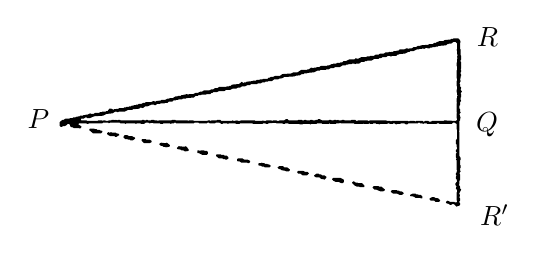
\begin{tikzpicture}[x=0.00744559cm,y=-0.00744559cm]
\fill[even odd rule] (709,311) -- (709,313) -- (711,315) -- (717,315) -- (719,317) -- (725,317) -- (727,315) -- (727,314) -- (724,311) -- (718,310) -- (717,309) -- (713,309) -- cycle
(676,305) -- (676,307) -- (682,308) -- (685,310) -- (693,310) -- (694,311) -- (696,311) -- (697,310) -- (697,308) -- (694,305) -- (690,305) -- (689,304) -- (686,304) -- (685,303) -- (680,303) -- cycle
(643,299) -- (643,300) -- (647,303) -- (654,303) -- (658,305) -- (662,305) -- (665,303) -- (665,302) -- (663,300) -- (661,299) -- (658,299) -- (657,298) -- (654,298) -- (653,297) -- (645,297) -- cycle
(612,292) -- (612,293) -- (615,296) -- (618,296) -- (625,299) -- (630,299) -- (633,297) -- (633,296) -- (627,291) -- (623,291) -- (622,290) -- (614,290) -- cycle
(577,284) -- (577,285) -- (581,289) -- (585,291) -- (589,291) -- (590,292) -- (597,292) -- (598,291) -- (598,289) -- (594,285) -- (587,285) -- (586,284) -- (583,284) -- (580,282) -- (579,282) -- cycle
(543,278) -- (543,279) -- (545,281) -- (549,283) -- (554,283) -- (558,285) -- (561,285) -- (563,283) -- (563,280) -- (561,278) -- (557,276) -- (545,276) -- cycle
(512,272) -- (512,273) -- (515,275) -- (521,275) -- (523,277) -- (525,278) -- (528,278) -- (529,279) -- (530,279) -- (533,276) -- (533,274) -- (530,272) -- (526,272) -- (524,270) -- (521,270) -- (520,269) -- (516,269) -- cycle
(483,266) -- (485,269) -- (489,269) -- (493,272) -- (500,272) -- (503,269) -- (503,268) -- (501,266) -- (497,266) -- (493,264) -- (485,264) -- cycle
(450,258) -- (450,259) -- (452,261) -- (454,261) -- (457,263) -- (463,264) -- (464,265) -- (469,265) -- (471,263) -- (471,262) -- (466,258) -- (461,258) -- (459,256) -- (453,256) -- cycle
(417,252) -- (417,254) -- (418,255) -- (420,255) -- (424,257) -- (427,257) -- (428,258) -- (436,258) -- (438,256) -- (438,255) -- (435,253) -- (433,253) -- (432,252) -- (428,252) -- (427,251) -- (424,251) -- (423,250) -- (421,251) -- (418,251) -- cycle
(381,244) -- (381,247) -- (382,248) -- (385,248) -- (388,250) -- (398,250) -- (399,251) -- (401,251) -- (403,249) -- (403,247) -- (399,245) -- (393,245) -- (390,243) -- (382,243) -- cycle
(345,237) -- (345,239) -- (350,243) -- (356,243) -- (357,244) -- (360,244) -- (361,245) -- (363,245) -- (366,243) -- (366,241) -- (363,238) -- (359,238) -- (358,237) -- (354,237) -- (353,236) -- (346,236) -- cycle
(313,230) -- (313,233) -- (314,234) -- (316,234) -- (322,237) -- (329,237) -- (331,235) -- (331,232) -- (329,230) -- (325,230) -- (324,229) -- (319,229) -- (318,230) -- (314,229) -- cycle
(278,225) -- (279,227) -- (285,228) -- (286,229) -- (289,229) -- (292,231) -- (298,230) -- (298,227) -- (296,225) -- (296,224) -- (293,222) -- (291,223) -- (281,222) -- cycle
(248,218) -- (248,219) -- (250,221) -- (254,222) -- (255,223) -- (258,223) -- (259,224) -- (265,223) -- (266,222) -- (266,220) -- (261,216) -- (259,217) -- (251,216) -- cycle
(218,211) -- (218,213) -- (222,217) -- (231,217) -- (235,215) -- (235,213) -- (232,211) -- (226,211) -- (225,210) -- (219,210) -- cycle
(187,206) -- (187,207) -- (190,210) -- (194,210) -- (195,211) -- (198,211) -- (199,212) -- (203,212) -- (207,209) -- (207,208) -- (205,206) -- (203,206) -- (202,205) -- (197,205) -- (193,203) -- (189,203) -- cycle
(159,200) -- (159,201) -- (161,203) -- (165,205) -- (172,205) -- (173,206) -- (175,206) -- (180,203) -- (179,201) -- (175,200) -- (174,199) -- (167,199) -- (166,198) -- (163,199) -- (161,198) -- cycle
(129,193) -- (129,195) -- (135,200) -- (149,200) -- (151,198) -- (151,196) -- (147,195) -- (146,194) -- (142,194) -- (141,193) -- (138,193) -- (137,192) -- (130,192) -- cycle
(762,44) -- (761,43) -- (761,41) -- (758,38) -- (750,38) -- (749,39) -- (746,39) -- (745,40) -- (735,41) -- (732,43) -- (725,43) -- (724,44) -- (722,44) -- (720,46) -- (717,46) -- (714,48) -- (708,48) -- (707,49) -- (694,50) -- (693,51) -- (689,51) -- (686,53) -- (682,53) -- (679,55) -- (675,55) -- (674,56) -- (670,55) -- (666,57) -- (658,57) -- (656,59) -- (653,59) -- (652,60) -- (648,60) -- (647,61) -- (644,61) -- (643,62) -- (641,61) -- (639,62) -- (634,62) -- (631,64) -- (625,64) -- (622,66) -- (617,66) -- (614,68) -- (608,68) -- (607,69) -- (602,69) -- (601,70) -- (593,70) -- (587,73) -- (583,72) -- (581,74) -- (572,74) -- (566,77) -- (562,77) -- (560,79) -- (557,79) -- (556,80) -- (551,80) -- (550,81) -- (545,81) -- (544,82) -- (542,82) -- (538,84) -- (535,84) -- (534,85) -- (524,85) -- (521,87) -- (517,87) -- (516,88) -- (512,88) -- (511,89) -- (507,88) -- (503,91) -- (501,91) -- (500,92) -- (490,92) -- (484,96) -- (477,96) -- (473,98) -- (458,99) -- (454,102) -- (446,102) -- (442,104) -- (438,104) -- (437,105) -- (435,105) -- (433,107) -- (425,107) -- (424,108) -- (420,108) -- (419,109) -- (414,109) -- (413,110) -- (408,110) -- (407,111) -- (397,112) -- (396,113) -- (393,113) -- (392,114) -- (391,114) -- (389,112) -- (384,116) -- (372,117) -- (370,119) -- (368,119) -- (367,120) -- (363,120) -- (362,121) -- (350,121) -- (347,123) -- (343,123) -- (340,125) -- (337,125) -- (333,127) -- (324,127) -- (321,129) -- (318,129) -- (314,131) -- (310,131) -- (306,133) -- (299,133) -- (298,134) -- (294,133) -- (293,134) -- (290,134) -- (289,135) -- (286,135) -- (285,136) -- (280,136) -- (279,137) -- (276,137) -- (271,140) -- (266,140) -- (265,141) -- (262,141) -- (258,143) -- (252,143) -- (251,144) -- (243,145) -- (242,146) -- (238,145) -- (234,147) -- (225,147) -- (224,148) -- (221,148) -- (217,150) -- (213,150) -- (212,151) -- (209,151) -- (208,152) -- (205,152) -- (204,153) -- (201,153) -- (200,154) -- (197,154) -- (196,155) -- (192,155) -- (191,156) -- (188,156) -- (187,157) -- (180,157) -- (179,158) -- (171,159) -- (170,160) -- (166,158) -- (163,158) -- (160,162) -- (158,162) -- (157,163) -- (151,163) -- (150,164) -- (147,164) -- (146,165) -- (139,165) -- (136,167) -- (132,167) -- (130,166) -- (126,168) -- (123,168) -- (122,169) -- (119,169) -- (118,170) -- (113,170) -- (112,171) -- (106,172) -- (105,173) -- (101,173) -- (100,174) -- (96,174) -- (95,175) -- (88,175) -- (85,177) -- (83,177) -- (78,181) -- (78,187) -- (80,189) -- (82,189) -- (83,188) -- (86,188) -- (90,186) -- (92,184) -- (94,184) -- (96,186) -- (96,188) -- (99,190) -- (101,190) -- (102,191) -- (111,191) -- (113,192) -- (115,190) -- (115,188) -- (110,185) -- (111,183) -- (124,183) -- (125,184) -- (127,184) -- (128,183) -- (151,183) -- (152,182) -- (161,182) -- (162,183) -- (164,182) -- (181,182) -- (182,183) -- (189,183) -- (190,184) -- (192,183) -- (207,183) -- (208,184) -- (210,183) -- (216,183) -- (217,184) -- (222,184) -- (225,182) -- (230,182) -- (231,183) -- (237,182) -- (238,183) -- (249,183) -- (250,184) -- (254,184) -- (255,183) -- (266,183) -- (268,184) -- (269,183) -- (273,183) -- (274,182) -- (276,182) -- (277,183) -- (307,183) -- (308,182) -- (315,182) -- (316,183) -- (329,183) -- (330,182) -- (333,182) -- (334,183) -- (343,183) -- (344,182) -- (351,182) -- (354,184) -- (356,184) -- (357,183) -- (364,183) -- (365,184) -- (367,183) -- (378,183) -- (379,184) -- (385,184) -- (386,183) -- (407,183) -- (408,184) -- (424,184) -- (425,183) -- (429,183) -- (430,184) -- (433,184) -- (434,183) -- (447,182) -- (448,183) -- (458,183) -- (459,184) -- (462,184) -- (463,183) -- (468,183) -- (469,184) -- (487,184) -- (488,185) -- (492,185) -- (493,184) -- (504,184) -- (506,185) -- (507,184) -- (516,184) -- (517,183) -- (525,183) -- (526,184) -- (537,184) -- (538,183) -- (540,184) -- (549,184) -- (550,183) -- (555,183) -- (556,182) -- (558,183) -- (580,183) -- (581,184) -- (595,184) -- (596,183) -- (597,184) -- (605,184) -- (606,183) -- (608,184) -- (612,184) -- (613,183) -- (617,183) -- (618,184) -- (622,184) -- (623,185) -- (625,184) -- (637,184) -- (638,183) -- (640,183) -- (641,184) -- (646,184) -- (647,183) -- (649,183) -- (652,185) -- (654,184) -- (659,184) -- (660,183) -- (666,183) -- (669,185) -- (671,185) -- (673,183) -- (689,183) -- (690,182) -- (692,182) -- (693,183) -- (697,183) -- (698,184) -- (700,183) -- (704,183) -- (705,184) -- (721,184) -- (722,183) -- (725,183) -- (726,184) -- (747,184) -- (749,182) -- (752,182) -- (755,184) -- (755,193) -- (756,194) -- (756,209) -- (754,212) -- (754,218) -- (755,219) -- (755,223) -- (756,224) -- (756,226) -- (754,229) -- (754,231) -- (755,232) -- (755,234) -- (754,235) -- (754,241) -- (755,243) -- (754,245) -- (755,246) -- (755,262) -- (756,263) -- (755,267) -- (754,268) -- (754,271) -- (755,272) -- (754,274) -- (754,277) -- (755,278) -- (756,282) -- (753,286) -- (753,288) -- (755,290) -- (754,294) -- (756,297) -- (756,300) -- (755,301) -- (755,314) -- (756,315) -- (756,317) -- (755,318) -- (752,318) -- (751,317) -- (744,317) -- (740,315) -- (738,316) -- (737,318) -- (739,320) -- (741,320) -- (744,322) -- (746,322) -- (747,321) -- (751,321) -- (755,325) -- (756,325) -- (757,324) -- (759,324) -- (761,322) -- (761,319) -- (760,318) -- (760,316) -- (761,315) -- (761,311) -- (760,310) -- (761,305) -- (760,304) -- (760,302) -- (763,296) -- (761,294) -- (761,291) -- (759,288) -- (760,286) -- (760,281) -- (761,280) -- (761,270) -- (760,268) -- (762,265) -- (761,263) -- (761,260) -- (762,259) -- (762,255) -- (761,254) -- (761,246) -- (762,245) -- (762,242) -- (760,239) -- (760,198) -- (759,197) -- (760,195) -- (760,179) -- (761,178) -- (761,175) -- (762,174) -- (760,167) -- (762,165) -- (762,164) -- (761,163) -- (761,159) -- (760,158) -- (760,153) -- (761,152) -- (761,147) -- (763,145) -- (762,143) -- (762,139) -- (763,138) -- (763,134) -- (762,132) -- (764,129) -- (764,128) -- (762,126) -- (763,122) -- (761,120) -- (761,116) -- (760,115) -- (762,111) -- (761,107) -- (762,106) -- (762,103) -- (763,102) -- (763,100) -- (762,99) -- (762,96) -- (763,95) -- (763,92) -- (762,91) -- (763,89) -- (763,79) -- (762,78) -- (762,75) -- (763,74) -- (763,68) -- (762,67) -- (762,57) -- (761,56) -- (761,46) -- cycle
(756,47) -- (756,56) -- (755,58) -- (756,59) -- (756,65) -- (757,66) -- (756,70) -- (757,72) -- (756,73) -- (756,79) -- (755,80) -- (755,85) -- (756,86) -- (756,92) -- (755,93) -- (755,106) -- (756,107) -- (756,110) -- (755,111) -- (755,119) -- (756,120) -- (756,125) -- (755,126) -- (755,130) -- (756,131) -- (756,134) -- (757,136) -- (756,137) -- (756,140) -- (755,141) -- (755,147) -- (756,148) -- (755,150) -- (755,164) -- (756,165) -- (755,167) -- (755,174) -- (756,175) -- (756,177) -- (754,179) -- (734,178) -- (733,179) -- (713,179) -- (712,180) -- (708,180) -- (707,179) -- (701,179) -- (700,180) -- (698,180) -- (697,179) -- (686,179) -- (685,180) -- (683,179) -- (675,179) -- (674,180) -- (672,179) -- (645,179) -- (643,180) -- (642,179) -- (636,179) -- (635,178) -- (607,178) -- (606,179) -- (604,179) -- (603,178) -- (587,178) -- (586,179) -- (584,179) -- (582,177) -- (576,177) -- (575,178) -- (564,178) -- (563,177) -- (560,177) -- (559,178) -- (554,178) -- (553,177) -- (551,178) -- (549,177) -- (546,177) -- (545,178) -- (542,178) -- (541,177) -- (538,177) -- (537,178) -- (526,178) -- (522,176) -- (519,176) -- (518,177) -- (515,177) -- (514,178) -- (510,178) -- (509,177) -- (506,177) -- (505,178) -- (499,178) -- (498,177) -- (496,177) -- (495,178) -- (492,178) -- (491,177) -- (485,177) -- (484,178) -- (469,178) -- (467,176) -- (464,176) -- (461,178) -- (453,178) -- (452,179) -- (449,179) -- (448,178) -- (442,178) -- (441,179) -- (439,178) -- (431,178) -- (430,179) -- (426,179) -- (425,178) -- (423,179) -- (412,179) -- (411,178) -- (387,178) -- (386,179) -- (382,179) -- (381,178) -- (375,179) -- (373,178) -- (372,179) -- (354,179) -- (352,177) -- (347,177) -- (346,178) -- (337,178) -- (336,179) -- (334,178) -- (331,178) -- (330,179) -- (307,179) -- (306,178) -- (299,178) -- (297,179) -- (296,178) -- (276,178) -- (275,177) -- (270,177) -- (269,178) -- (247,178) -- (246,179) -- (244,178) -- (240,178) -- (239,177) -- (235,177) -- (234,178) -- (229,178) -- (228,177) -- (226,177) -- (225,178) -- (223,178) -- (222,177) -- (219,177) -- (218,178) -- (182,178) -- (181,177) -- (178,177) -- (176,178) -- (174,177) -- (172,178) -- (171,177) -- (167,177) -- (166,178) -- (162,178) -- (161,179) -- (157,179) -- (156,178) -- (153,178) -- (152,179) -- (150,178) -- (144,178) -- (143,179) -- (125,179) -- (124,178) -- (115,178) -- (114,177) -- (115,175) -- (119,175) -- (122,173) -- (124,173) -- (125,174) -- (130,174) -- (137,171) -- (152,170) -- (158,167) -- (168,166) -- (173,163) -- (175,163) -- (176,164) -- (178,164) -- (179,163) -- (189,163) -- (195,160) -- (202,160) -- (203,159) -- (214,158) -- (216,156) -- (220,157) -- (224,154) -- (228,154) -- (235,151) -- (239,151) -- (240,152) -- (242,152) -- (244,150) -- (249,150) -- (250,149) -- (257,149) -- (258,148) -- (262,148) -- (264,146) -- (270,146) -- (272,144) -- (276,144) -- (277,143) -- (280,143) -- (281,142) -- (287,142) -- (288,141) -- (293,141) -- (294,140) -- (307,139) -- (309,137) -- (311,136) -- (314,136) -- (315,135) -- (319,135) -- (320,134) -- (328,134) -- (329,133) -- (335,133) -- (337,131) -- (339,131) -- (340,130) -- (346,130) -- (350,128) -- (359,128) -- (362,126) -- (369,126) -- (373,124) -- (379,124) -- (382,122) -- (386,122) -- (389,120) -- (394,120) -- (398,118) -- (402,118) -- (405,116) -- (415,116) -- (416,115) -- (421,115) -- (424,113) -- (428,113) -- (429,112) -- (433,112) -- (434,111) -- (440,111) -- (444,108) -- (451,108) -- (452,107) -- (458,106) -- (461,104) -- (479,103) -- (480,102) -- (488,101) -- (491,99) -- (494,99) -- (495,98) -- (500,98) -- (501,97) -- (512,96) -- (518,93) -- (522,93) -- (523,92) -- (532,92) -- (533,91) -- (537,91) -- (540,89) -- (545,89) -- (548,87) -- (556,87) -- (561,84) -- (566,84) -- (567,83) -- (570,83) -- (571,82) -- (576,82) -- (577,81) -- (581,81) -- (582,82) -- (584,81) -- (589,81) -- (593,78) -- (598,78) -- (599,77) -- (602,77) -- (603,76) -- (610,76) -- (615,73) -- (622,73) -- (623,72) -- (626,72) -- (629,70) -- (635,70) -- (638,68) -- (641,68) -- (642,69) -- (644,69) -- (645,68) -- (652,68) -- (654,66) -- (656,66) -- (657,65) -- (667,64) -- (673,61) -- (675,61) -- (676,60) -- (681,60) -- (687,57) -- (691,57) -- (692,56) -- (696,56) -- (697,55) -- (700,56) -- (704,54) -- (706,55) -- (709,55) -- (710,54) -- (713,54) -- (714,53) -- (719,53) -- (720,52) -- (723,52) -- (724,51) -- (737,50) -- (739,48) -- (741,48) -- (742,47) -- (746,47) -- (750,44) -- (753,44) -- cycle;
\node[inner sep=0pt,font=\fontsize{10}{12}\selectfont] at (42,176) {$P$};
\node[inner sep=0pt,font=\fontsize{10}{12}\selectfont] at (808,36) {$R$};
\node[inner sep=0pt,font=\fontsize{10}{12}\selectfont] at (807,185) {$Q$};
\node[inner sep=0pt,font=\fontsize{10}{12}\selectfont] at (820,340) {$R'$};
\end{tikzpicture}


Fig. 2.
\end{minipage}\end{center}

\Needspace{30\baselineskip}\noindent 2. Es sei $ABCD$ ein Viereck mit der unendlich kleinen Grundlinie $AB=du$. Die Winkel in $A$ und $B$ seien rechte und $AD=BC=y$. Dann ist die L\"ange der vierten Seite $CD=du'$ proportional $du$, und der Proportionalit\"atsfactor h\"angt nur von $y$ ab. Man hat daher

\[
\tag*{(B)} du' = g(y)\,du.
\]

\begin{center}\begin{minipage}{\linewidth}\centering
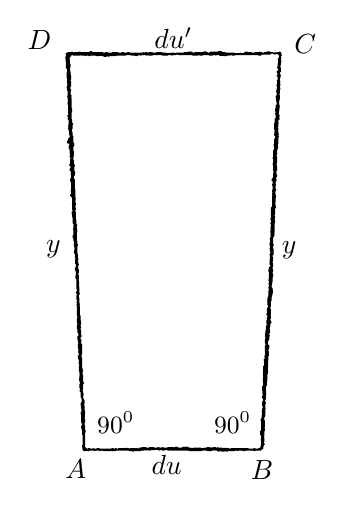
\begin{tikzpicture}[x=0.00658784cm,y=-0.00658784cm]
\fill[even odd rule] (103,61) -- (98,64) -- (99,66) -- (99,69) -- (98,70) -- (98,75) -- (99,76) -- (98,78) -- (99,80) -- (99,92) -- (101,94) -- (101,99) -- (100,100) -- (100,110) -- (101,111) -- (101,122) -- (102,123) -- (100,130) -- (101,131) -- (101,135) -- (102,136) -- (102,145) -- (101,147) -- (102,148) -- (102,153) -- (103,154) -- (103,156) -- (102,157) -- (102,162) -- (103,163) -- (103,173) -- (104,174) -- (103,176) -- (103,179) -- (104,181) -- (101,184) -- (103,186) -- (102,190) -- (104,192) -- (104,201) -- (103,202) -- (104,206) -- (103,207) -- (103,209) -- (104,210) -- (104,213) -- (105,214) -- (105,220) -- (106,221) -- (106,225) -- (103,228) -- (103,230) -- (101,233) -- (101,237) -- (104,237) -- (106,239) -- (104,243) -- (104,246) -- (106,249) -- (106,256) -- (107,257) -- (106,263) -- (108,265) -- (107,267) -- (107,276) -- (105,278) -- (105,279) -- (108,282) -- (108,284) -- (106,286) -- (106,289) -- (109,292) -- (109,294) -- (108,295) -- (109,302) -- (107,306) -- (107,309) -- (109,313) -- (109,326) -- (108,327) -- (109,334) -- (107,336) -- (107,338) -- (111,342) -- (111,352) -- (110,354) -- (111,355) -- (111,365) -- (112,367) -- (110,369) -- (110,372) -- (111,373) -- (111,379) -- (112,380) -- (112,391) -- (114,393) -- (113,395) -- (113,401) -- (112,402) -- (113,404) -- (113,413) -- (112,414) -- (112,419) -- (113,420) -- (113,424) -- (115,428) -- (114,430) -- (114,435) -- (115,436) -- (115,439) -- (116,441) -- (115,442) -- (114,448) -- (117,451) -- (116,453) -- (116,457) -- (117,458) -- (117,460) -- (116,461) -- (117,466) -- (116,468) -- (118,470) -- (118,475) -- (116,477) -- (116,481) -- (118,484) -- (118,491) -- (117,492) -- (117,496) -- (119,499) -- (119,517) -- (120,518) -- (120,521) -- (118,524) -- (118,525) -- (120,527) -- (120,529) -- (119,530) -- (119,537) -- (120,538) -- (120,542) -- (119,543) -- (120,545) -- (120,547) -- (119,548) -- (120,550) -- (120,570) -- (121,571) -- (121,573) -- (120,574) -- (120,582) -- (121,583) -- (121,586) -- (120,587) -- (120,594) -- (121,595) -- (121,601) -- (123,604) -- (123,607) -- (121,609) -- (121,615) -- (122,616) -- (122,620) -- (123,621) -- (123,623) -- (122,624) -- (122,632) -- (123,633) -- (123,637) -- (122,639) -- (124,642) -- (124,644) -- (122,646) -- (122,651) -- (124,655) -- (124,658) -- (123,659) -- (124,663) -- (125,664) -- (124,666) -- (124,676) -- (125,677) -- (125,681) -- (126,682) -- (125,684) -- (125,689) -- (124,690) -- (125,696) -- (126,697) -- (126,700) -- (125,701) -- (125,708) -- (126,709) -- (126,712) -- (125,714) -- (127,716) -- (127,725) -- (129,729) -- (129,735) -- (127,738) -- (129,753) -- (127,756) -- (127,758) -- (128,759) -- (128,774) -- (129,775) -- (129,778) -- (130,779) -- (128,783) -- (128,785) -- (129,786) -- (129,789) -- (130,790) -- (130,798) -- (131,799) -- (131,818) -- (130,819) -- (131,828) -- (135,830) -- (138,830) -- (139,829) -- (141,830) -- (143,830) -- (144,829) -- (153,829) -- (154,830) -- (156,829) -- (163,829) -- (164,830) -- (166,830) -- (167,829) -- (170,829) -- (171,830) -- (185,830) -- (186,829) -- (188,830) -- (194,830) -- (195,829) -- (220,829) -- (221,830) -- (226,830) -- (227,831) -- (229,831) -- (230,830) -- (243,830) -- (244,829) -- (249,829) -- (250,828) -- (252,828) -- (253,829) -- (255,828) -- (261,829) -- (262,828) -- (271,828) -- (272,827) -- (278,828) -- (279,829) -- (281,828) -- (284,828) -- (285,829) -- (288,829) -- (289,828) -- (294,828) -- (295,829) -- (299,829) -- (300,828) -- (302,829) -- (308,829) -- (309,828) -- (310,829) -- (335,829) -- (336,830) -- (355,830) -- (356,829) -- (360,830) -- (361,829) -- (365,829) -- (366,828) -- (368,829) -- (371,829) -- (372,830) -- (379,830) -- (380,829) -- (385,828) -- (386,829) -- (390,829) -- (393,831) -- (395,830) -- (398,830) -- (399,831) -- (404,831) -- (405,830) -- (407,830) -- (408,831) -- (410,831) -- (411,830) -- (424,830) -- (425,829) -- (428,829) -- (429,830) -- (431,829) -- (439,829) -- (440,830) -- (444,830) -- (445,829) -- (460,829) -- (461,830) -- (463,830) -- (464,829) -- (474,829) -- (479,825) -- (480,819) -- (482,817) -- (482,816) -- (480,814) -- (481,812) -- (481,804) -- (480,802) -- (481,801) -- (481,792) -- (482,791) -- (482,786) -- (481,785) -- (482,784) -- (482,771) -- (481,770) -- (481,765) -- (483,763) -- (483,749) -- (484,748) -- (483,746) -- (483,739) -- (484,738) -- (484,736) -- (483,735) -- (483,731) -- (484,730) -- (484,722) -- (485,721) -- (485,719) -- (484,718) -- (485,716) -- (484,714) -- (484,707) -- (486,703) -- (486,695) -- (487,694) -- (487,682) -- (488,681) -- (488,677) -- (489,676) -- (488,674) -- (489,647) -- (490,646) -- (490,638) -- (489,637) -- (489,635) -- (490,634) -- (490,631) -- (491,630) -- (491,626) -- (488,624) -- (488,619) -- (491,614) -- (491,609) -- (492,608) -- (492,607) -- (490,605) -- (492,601) -- (492,596) -- (491,594) -- (492,593) -- (492,590) -- (493,589) -- (493,584) -- (495,582) -- (493,578) -- (493,575) -- (494,574) -- (494,569) -- (493,568) -- (494,566) -- (494,556) -- (493,555) -- (493,552) -- (494,551) -- (494,541) -- (495,540) -- (495,533) -- (496,532) -- (497,526) -- (498,525) -- (497,516) -- (495,513) -- (495,511) -- (496,510) -- (496,505) -- (497,504) -- (497,495) -- (498,494) -- (498,488) -- (497,487) -- (497,485) -- (498,484) -- (498,480) -- (497,479) -- (497,475) -- (498,474) -- (498,468) -- (497,467) -- (497,465) -- (498,464) -- (498,456) -- (497,455) -- (497,453) -- (499,451) -- (499,440) -- (498,439) -- (498,435) -- (499,434) -- (499,431) -- (498,430) -- (498,419) -- (501,413) -- (501,411) -- (500,410) -- (501,408) -- (501,391) -- (502,390) -- (502,386) -- (501,385) -- (502,378) -- (501,377) -- (501,375) -- (502,374) -- (502,363) -- (504,360) -- (503,358) -- (503,354) -- (502,353) -- (502,351) -- (503,350) -- (503,342) -- (504,341) -- (502,330) -- (504,328) -- (504,326) -- (503,325) -- (503,318) -- (504,317) -- (503,315) -- (503,312) -- (505,308) -- (504,306) -- (504,303) -- (506,300) -- (506,298) -- (504,296) -- (505,294) -- (504,291) -- (506,289) -- (506,280) -- (505,279) -- (505,276) -- (506,275) -- (506,263) -- (505,262) -- (505,259) -- (506,258) -- (506,253) -- (505,251) -- (507,249) -- (507,246) -- (508,245) -- (507,239) -- (508,238) -- (508,226) -- (509,225) -- (509,223) -- (508,222) -- (509,220) -- (509,218) -- (508,217) -- (508,208) -- (507,206) -- (508,205) -- (508,199) -- (509,198) -- (508,197) -- (508,193) -- (511,190) -- (510,189) -- (510,186) -- (511,184) -- (509,180) -- (511,165) -- (510,164) -- (510,160) -- (509,158) -- (510,157) -- (510,153) -- (511,152) -- (511,144) -- (510,142) -- (511,141) -- (511,134) -- (512,133) -- (512,130) -- (511,129) -- (511,127) -- (512,126) -- (512,123) -- (511,122) -- (512,120) -- (511,112) -- (512,111) -- (513,105) -- (511,103) -- (511,101) -- (513,99) -- (513,91) -- (512,90) -- (512,87) -- (513,86) -- (513,81) -- (514,80) -- (514,77) -- (513,76) -- (513,74) -- (514,73) -- (513,70) -- (515,67) -- (514,65) -- (514,62) -- (511,60) -- (509,61) -- (499,62) -- (498,61) -- (493,61) -- (490,59) -- (488,60) -- (485,60) -- (484,61) -- (481,61) -- (480,62) -- (477,62) -- (476,61) -- (473,61) -- (472,60) -- (470,61) -- (463,61) -- (462,62) -- (457,62) -- (456,61) -- (449,61) -- (448,60) -- (445,60) -- (441,63) -- (436,63) -- (435,62) -- (433,63) -- (424,63) -- (423,62) -- (407,62) -- (406,61) -- (401,61) -- (398,59) -- (393,59) -- (392,60) -- (377,60) -- (375,62) -- (373,62) -- (367,59) -- (366,60) -- (363,60) -- (362,61) -- (347,61) -- (346,62) -- (344,62) -- (341,60) -- (334,60) -- (333,61) -- (327,61) -- (326,62) -- (311,62) -- (310,63) -- (308,63) -- (307,62) -- (293,63) -- (292,62) -- (285,62) -- (284,61) -- (274,61) -- (273,62) -- (266,62) -- (265,61) -- (259,61) -- (258,62) -- (252,61) -- (250,62) -- (248,61) -- (247,62) -- (240,62) -- (239,63) -- (237,62) -- (230,62) -- (228,63) -- (227,62) -- (222,62) -- (221,61) -- (217,61) -- (216,62) -- (211,62) -- (210,61) -- (207,61) -- (206,62) -- (200,62) -- (199,61) -- (188,61) -- (187,62) -- (180,62) -- (179,61) -- (175,61) -- (174,62) -- (171,62) -- (170,61) -- (150,61) -- (148,59) -- (146,59) -- (144,61) -- (127,61) -- (126,60) -- (124,60) -- (123,61) -- (115,61) -- (114,62) -- (111,60) -- (109,61) -- cycle
(507,65) -- (509,67) -- (509,72) -- (507,74) -- (508,82) -- (507,83) -- (507,89) -- (506,90) -- (506,92) -- (508,94) -- (508,95) -- (505,98) -- (505,100) -- (507,103) -- (507,104) -- (505,106) -- (505,107) -- (507,109) -- (507,114) -- (505,116) -- (506,118) -- (506,122) -- (505,123) -- (505,128) -- (506,130) -- (505,131) -- (505,135) -- (504,136) -- (504,138) -- (505,139) -- (505,144) -- (503,146) -- (504,156) -- (505,157) -- (505,162) -- (503,164) -- (503,169) -- (502,170) -- (502,175) -- (503,176) -- (503,178) -- (502,179) -- (502,181) -- (503,182) -- (503,188) -- (501,190) -- (501,197) -- (500,198) -- (500,210) -- (501,211) -- (500,221) -- (502,224) -- (502,226) -- (500,229) -- (500,238) -- (499,239) -- (499,242) -- (500,243) -- (500,248) -- (498,251) -- (498,263) -- (497,264) -- (497,266) -- (499,269) -- (498,271) -- (498,275) -- (497,276) -- (497,278) -- (498,279) -- (498,290) -- (499,291) -- (499,293) -- (498,294) -- (498,302) -- (495,306) -- (495,308) -- (497,310) -- (497,315) -- (496,316) -- (496,318) -- (497,319) -- (497,326) -- (496,327) -- (496,330) -- (497,332) -- (496,333) -- (496,335) -- (497,337) -- (496,338) -- (496,358) -- (494,361) -- (494,381) -- (493,382) -- (493,384) -- (494,385) -- (494,389) -- (493,390) -- (493,392) -- (494,393) -- (494,398) -- (493,399) -- (493,401) -- (494,402) -- (493,404) -- (493,409) -- (494,411) -- (493,412) -- (493,414) -- (494,416) -- (492,419) -- (492,423) -- (493,425) -- (492,426) -- (492,429) -- (491,430) -- (491,432) -- (492,433) -- (492,438) -- (491,440) -- (492,441) -- (492,445) -- (493,446) -- (493,448) -- (491,451) -- (492,453) -- (491,470) -- (493,472) -- (493,473) -- (490,476) -- (490,479) -- (489,480) -- (489,484) -- (490,485) -- (490,498) -- (489,499) -- (489,501) -- (490,502) -- (490,506) -- (489,507) -- (490,509) -- (490,512) -- (489,513) -- (489,516) -- (490,517) -- (490,520) -- (489,521) -- (489,531) -- (487,535) -- (487,548) -- (488,549) -- (488,552) -- (486,556) -- (486,564) -- (485,565) -- (485,567) -- (487,569) -- (487,571) -- (486,572) -- (486,577) -- (485,578) -- (485,584) -- (486,586) -- (484,590) -- (484,597) -- (483,598) -- (484,599) -- (483,600) -- (483,603) -- (482,604) -- (483,606) -- (482,608) -- (483,610) -- (483,613) -- (482,614) -- (482,622) -- (483,623) -- (483,626) -- (482,627) -- (482,638) -- (483,640) -- (482,642) -- (483,644) -- (481,647) -- (482,651) -- (480,653) -- (481,664) -- (479,666) -- (479,681) -- (478,682) -- (479,684) -- (479,690) -- (478,691) -- (479,703) -- (477,705) -- (477,714) -- (478,715) -- (477,719) -- (478,720) -- (478,722) -- (476,726) -- (479,730) -- (479,732) -- (477,735) -- (477,742) -- (478,743) -- (478,747) -- (477,748) -- (477,752) -- (476,753) -- (477,759) -- (476,760) -- (476,765) -- (474,769) -- (474,772) -- (475,773) -- (475,789) -- (473,791) -- (473,798) -- (475,800) -- (475,807) -- (474,808) -- (475,810) -- (475,818) -- (474,819) -- (474,822) -- (472,824) -- (470,824) -- (469,825) -- (464,825) -- (463,824) -- (461,824) -- (460,825) -- (451,825) -- (450,824) -- (417,824) -- (416,825) -- (414,825) -- (413,824) -- (393,823) -- (392,822) -- (390,823) -- (388,823) -- (387,822) -- (383,822) -- (382,823) -- (371,822) -- (370,823) -- (366,823) -- (365,824) -- (360,824) -- (359,823) -- (345,823) -- (344,824) -- (341,824) -- (340,823) -- (336,823) -- (333,821) -- (323,822) -- (322,823) -- (316,823) -- (312,821) -- (310,821) -- (308,823) -- (306,822) -- (295,822) -- (294,823) -- (287,823) -- (286,822) -- (284,822) -- (283,823) -- (279,823) -- (278,822) -- (276,822) -- (275,823) -- (269,823) -- (268,822) -- (260,822) -- (259,823) -- (254,823) -- (253,822) -- (245,822) -- (244,823) -- (240,823) -- (238,825) -- (236,824) -- (223,824) -- (221,825) -- (220,824) -- (216,824) -- (215,823) -- (213,824) -- (200,824) -- (199,825) -- (197,825) -- (196,824) -- (194,824) -- (193,825) -- (191,825) -- (190,824) -- (187,824) -- (186,825) -- (164,825) -- (163,824) -- (159,824) -- (158,825) -- (153,825) -- (152,824) -- (150,825) -- (146,825) -- (145,824) -- (142,824) -- (141,825) -- (139,825) -- (136,822) -- (136,794) -- (137,793) -- (137,790) -- (136,789) -- (136,780) -- (135,779) -- (135,775) -- (136,774) -- (136,768) -- (135,767) -- (136,752) -- (135,751) -- (135,742) -- (134,741) -- (134,739) -- (135,738) -- (135,733) -- (132,727) -- (133,719) -- (132,718) -- (132,715) -- (131,714) -- (131,712) -- (132,711) -- (132,708) -- (131,706) -- (132,705) -- (132,701) -- (134,699) -- (134,698) -- (132,696) -- (132,683) -- (131,682) -- (131,677) -- (132,676) -- (132,674) -- (131,673) -- (131,670) -- (130,669) -- (130,650) -- (129,649) -- (129,644) -- (130,643) -- (130,624) -- (128,622) -- (129,616) -- (127,614) -- (127,611) -- (129,609) -- (129,607) -- (128,606) -- (128,597) -- (127,596) -- (127,594) -- (128,593) -- (128,590) -- (127,589) -- (127,587) -- (128,586) -- (128,579) -- (127,578) -- (127,569) -- (126,568) -- (126,551) -- (125,550) -- (126,546) -- (125,545) -- (125,535) -- (124,534) -- (124,529) -- (126,527) -- (125,525) -- (124,501) -- (123,500) -- (124,498) -- (124,491) -- (123,490) -- (123,487) -- (124,486) -- (124,480) -- (122,478) -- (123,476) -- (122,473) -- (124,471) -- (124,470) -- (123,469) -- (123,466) -- (122,465) -- (122,462) -- (123,461) -- (123,459) -- (122,458) -- (122,450) -- (121,449) -- (121,435) -- (122,434) -- (122,432) -- (121,431) -- (121,425) -- (120,424) -- (120,407) -- (121,406) -- (121,404) -- (120,403) -- (120,399) -- (119,397) -- (121,395) -- (121,394) -- (119,392) -- (119,384) -- (118,383) -- (118,369) -- (117,368) -- (117,366) -- (118,365) -- (118,361) -- (117,360) -- (117,357) -- (118,356) -- (118,351) -- (117,350) -- (118,342) -- (117,341) -- (117,326) -- (116,325) -- (116,307) -- (114,304) -- (114,301) -- (116,298) -- (117,292) -- (115,290) -- (115,282) -- (116,281) -- (116,279) -- (114,275) -- (114,269) -- (113,268) -- (113,263) -- (114,262) -- (114,252) -- (113,251) -- (113,244) -- (115,241) -- (115,238) -- (113,234) -- (113,223) -- (112,222) -- (112,216) -- (111,215) -- (111,209) -- (112,208) -- (112,201) -- (113,199) -- (111,197) -- (111,191) -- (110,190) -- (110,177) -- (111,176) -- (111,170) -- (110,169) -- (110,150) -- (109,149) -- (110,145) -- (108,142) -- (108,137) -- (109,136) -- (109,134) -- (107,130) -- (109,126) -- (109,118) -- (108,117) -- (108,115) -- (109,114) -- (109,105) -- (108,104) -- (108,99) -- (107,98) -- (107,90) -- (108,89) -- (108,85) -- (107,84) -- (106,72) -- (110,67) -- (112,67) -- (113,68) -- (125,68) -- (127,67) -- (128,68) -- (135,68) -- (136,69) -- (138,68) -- (142,68) -- (143,69) -- (145,69) -- (146,68) -- (156,68) -- (157,69) -- (167,68) -- (168,69) -- (171,69) -- (172,70) -- (177,70) -- (178,69) -- (182,70) -- (183,69) -- (189,69) -- (190,68) -- (192,69) -- (195,69) -- (196,68) -- (214,68) -- (215,67) -- (224,67) -- (225,68) -- (232,68) -- (233,69) -- (235,69) -- (239,67) -- (241,67) -- (242,68) -- (244,68) -- (245,67) -- (253,67) -- (254,68) -- (258,67) -- (259,68) -- (265,68) -- (266,67) -- (276,67) -- (277,66) -- (279,67) -- (284,67) -- (285,68) -- (295,68) -- (296,67) -- (302,67) -- (304,68) -- (305,67) -- (311,67) -- (312,66) -- (315,66) -- (316,67) -- (342,67) -- (343,68) -- (353,68) -- (354,67) -- (356,67) -- (357,68) -- (362,68) -- (363,67) -- (374,67) -- (375,68) -- (381,68) -- (382,67) -- (386,67) -- (388,68) -- (389,67) -- (394,67) -- (395,68) -- (408,69) -- (409,68) -- (415,68) -- (416,67) -- (418,67) -- (419,68) -- (424,68) -- (425,67) -- (469,67) -- (470,68) -- (474,68) -- (477,66) -- (492,66) -- (495,64) -- (498,64) -- (501,66) -- (503,65) -- cycle;
\node[inner sep=0pt,font=\fontsize{10}{12}\selectfont] at (48,37) {$D$};
\node[inner sep=0pt,font=\fontsize{10}{12}\selectfont] at (306,34) {$du'$};
\node[inner sep=0pt,font=\fontsize{10}{12}\selectfont] at (560,45) {$C$};
\node[inner sep=0pt,font=\fontsize{10}{12}\selectfont] at (75,441) {$y$};
\node[inner sep=0pt,font=\fontsize{10}{12}\selectfont] at (529,442) {$y$};
\node[inner sep=0pt,font=\fontsize{9}{11}\selectfont] at (195,775) {$90^{0}$};
\node[inner sep=0pt,font=\fontsize{9}{11}\selectfont] at (420,775) {$90^{0}$};
\node[inner sep=0pt,font=\fontsize{10}{12}\selectfont] at (118,865) {$A$};
\node[inner sep=0pt,font=\fontsize{10}{12}\selectfont] at (293,856) {$du$};
\node[inner sep=0pt,font=\fontsize{10}{12}\selectfont] at (477,866) {$B$};
\end{tikzpicture}


Fig. 3.
\end{minipage}\end{center}

\Needspace{37\baselineskip}\noindent 3. In dem rechtwinkligen Dreieck $ABC$ mit den Katheten $a,b$ und der Hypotenuse $c$ lasse man $b$ um ein unendlich kleines St\"uck $CC'=db$ wachsen, w\"ahrend der Winkel $A$ unver\"andert bleibt. Die Senkrechte $C'B'$, die in $C'$ auf $AC'$ errichtet ist, schneide $AB$ in $B'$, sodass ein rechtwinkliges Dreieck $AB'C'$ mit den Katheten $a+da, b+db$ und der Hypotenuse $c+dc$ entsteht. Macht man auf $C'B'$ \ $C'D=a$, so wird nach (B):

\[
BD = g(a)\,.\,db.
\]

\begin{center}\begin{minipage}{\linewidth}\centering
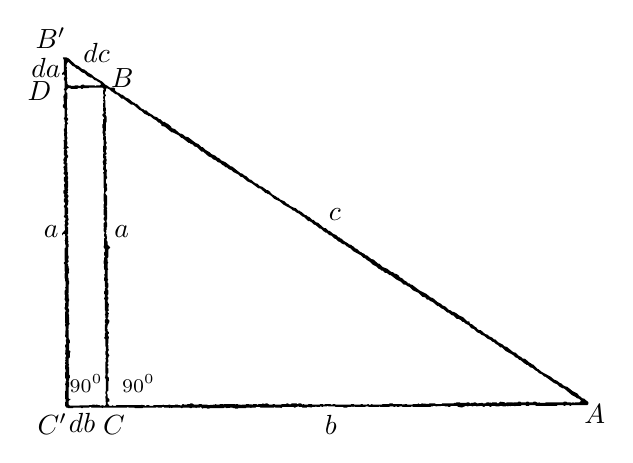
\begin{tikzpicture}[x=0.00740038cm,y=-0.00740038cm]
\fill[even odd rule] (75,75) -- (77,79) -- (77,98) -- (74,101) -- (74,104) -- (76,103) -- (78,105) -- (78,108) -- (77,109) -- (77,113) -- (78,114) -- (78,127) -- (77,128) -- (77,130) -- (78,131) -- (78,137) -- (76,141) -- (77,154) -- (75,156) -- (75,159) -- (78,162) -- (78,177) -- (77,178) -- (77,180) -- (78,181) -- (78,185) -- (79,186) -- (79,188) -- (78,189) -- (78,196) -- (77,197) -- (77,201) -- (78,202) -- (77,204) -- (78,215) -- (76,217) -- (77,219) -- (77,228) -- (76,230) -- (78,232) -- (77,234) -- (77,242) -- (78,243) -- (78,245) -- (76,249) -- (76,251) -- (77,252) -- (76,256) -- (78,258) -- (78,260) -- (76,262) -- (76,263) -- (77,264) -- (77,267) -- (78,269) -- (76,273) -- (79,277) -- (79,278) -- (77,280) -- (77,286) -- (79,290) -- (77,292) -- (78,301) -- (76,303) -- (76,307) -- (78,310) -- (77,312) -- (78,314) -- (78,316) -- (77,317) -- (77,322) -- (79,324) -- (79,326) -- (77,329) -- (77,331) -- (78,332) -- (78,345) -- (77,346) -- (77,348) -- (80,351) -- (78,356) -- (79,358) -- (79,360) -- (78,361) -- (79,370) -- (74,376) -- (74,380) -- (74,379) -- (76,377) -- (78,377) -- (79,378) -- (79,381) -- (80,382) -- (79,384) -- (79,387) -- (78,388) -- (79,390) -- (79,395) -- (80,396) -- (80,400) -- (78,402) -- (78,422) -- (79,424) -- (77,426) -- (77,428) -- (78,429) -- (78,441) -- (79,442) -- (79,444) -- (78,445) -- (78,453) -- (79,454) -- (79,458) -- (80,459) -- (80,468) -- (79,469) -- (80,472) -- (78,475) -- (78,481) -- (79,482) -- (78,490) -- (79,491) -- (80,495) -- (79,496) -- (79,502) -- (78,503) -- (78,506) -- (80,508) -- (80,510) -- (79,511) -- (79,530) -- (80,531) -- (79,532) -- (79,535) -- (80,536) -- (79,553) -- (81,556) -- (81,558) -- (80,559) -- (81,565) -- (79,568) -- (79,571) -- (80,572) -- (79,583) -- (81,586) -- (79,590) -- (80,592) -- (79,594) -- (80,596) -- (79,598) -- (79,600) -- (80,601) -- (79,603) -- (79,609) -- (80,610) -- (80,614) -- (79,615) -- (79,624) -- (81,628) -- (80,630) -- (80,633) -- (79,634) -- (79,636) -- (80,637) -- (80,646) -- (79,647) -- (79,660) -- (80,661) -- (80,665) -- (79,666) -- (79,672) -- (81,675) -- (83,675) -- (84,676) -- (92,676) -- (93,675) -- (106,675) -- (107,676) -- (109,676) -- (110,675) -- (120,675) -- (121,674) -- (123,674) -- (124,675) -- (141,675) -- (143,676) -- (144,675) -- (185,675) -- (187,674) -- (188,675) -- (198,675) -- (199,676) -- (212,676) -- (213,675) -- (235,675) -- (236,674) -- (238,675) -- (245,675) -- (246,674) -- (248,674) -- (249,675) -- (257,675) -- (258,676) -- (260,675) -- (262,676) -- (264,675) -- (277,675) -- (278,676) -- (280,676) -- (281,675) -- (292,675) -- (293,676) -- (296,676) -- (297,675) -- (302,675) -- (304,676) -- (305,675) -- (310,675) -- (312,674) -- (315,677) -- (316,676) -- (322,676) -- (323,677) -- (326,677) -- (327,676) -- (351,676) -- (352,675) -- (355,675) -- (356,676) -- (366,675) -- (367,676) -- (370,676) -- (371,677) -- (375,677) -- (376,676) -- (389,676) -- (390,675) -- (396,675) -- (398,676) -- (399,675) -- (406,675) -- (407,674) -- (413,674) -- (414,675) -- (437,675) -- (439,674) -- (440,675) -- (448,675) -- (450,676) -- (452,674) -- (471,674) -- (472,675) -- (474,675) -- (475,674) -- (480,673) -- (481,674) -- (485,674) -- (486,675) -- (494,675) -- (495,674) -- (502,675) -- (503,674) -- (508,674) -- (509,673) -- (511,674) -- (516,674) -- (517,673) -- (521,674) -- (522,673) -- (528,673) -- (529,672) -- (531,673) -- (542,673) -- (543,674) -- (556,674) -- (557,675) -- (563,675) -- (564,674) -- (570,674) -- (571,673) -- (573,674) -- (575,673) -- (577,674) -- (594,674) -- (595,673) -- (599,673) -- (600,674) -- (617,674) -- (618,673) -- (620,674) -- (635,674) -- (636,673) -- (642,673) -- (643,674) -- (645,674) -- (646,673) -- (648,673) -- (649,674) -- (652,674) -- (653,673) -- (657,673) -- (658,674) -- (672,674) -- (673,673) -- (675,673) -- (676,674) -- (706,674) -- (707,673) -- (710,673) -- (711,672) -- (714,672) -- (715,673) -- (730,672) -- (731,673) -- (736,673) -- (737,674) -- (739,674) -- (742,672) -- (751,672) -- (754,674) -- (760,675) -- (767,672) -- (769,673) -- (771,673) -- (772,672) -- (776,672) -- (777,673) -- (779,673) -- (780,672) -- (784,672) -- (785,673) -- (794,672) -- (797,674) -- (798,674) -- (800,672) -- (806,672) -- (808,674) -- (809,674) -- (812,672) -- (817,672) -- (818,673) -- (824,673) -- (825,672) -- (829,672) -- (830,673) -- (835,673) -- (836,672) -- (839,673) -- (841,672) -- (843,673) -- (844,672) -- (849,672) -- (851,673) -- (852,672) -- (861,672) -- (862,671) -- (869,671) -- (870,672) -- (875,672) -- (876,671) -- (886,671) -- (887,672) -- (923,672) -- (924,671) -- (934,671) -- (935,672) -- (937,672) -- (938,671) -- (944,671) -- (945,672) -- (947,672) -- (948,671) -- (975,671) -- (977,669) -- (977,666) -- (974,663) -- (973,663) -- (970,660) -- (966,659) -- (963,656) -- (962,656) -- (958,651) -- (950,647) -- (940,639) -- (938,639) -- (934,637) -- (931,634) -- (928,633) -- (923,629) -- (918,627) -- (912,622) -- (897,614) -- (891,609) -- (890,609) -- (882,601) -- (880,601) -- (878,599) -- (877,599) -- (869,592) -- (867,591) -- (864,591) -- (861,588) -- (857,586) -- (852,581) -- (848,580) -- (837,571) -- (833,570) -- (830,567) -- (822,563) -- (817,558) -- (815,558) -- (812,555) -- (807,553) -- (804,550) -- (800,549) -- (792,542) -- (789,542) -- (787,541) -- (784,537) -- (783,537) -- (777,532) -- (775,532) -- (773,530) -- (773,528) -- (772,527) -- (769,527) -- (762,520) -- (755,517) -- (750,513) -- (746,511) -- (744,511) -- (740,508) -- (738,508) -- (732,502) -- (727,500) -- (724,497) -- (718,494) -- (710,487) -- (706,486) -- (699,480) -- (687,474) -- (674,464) -- (672,464) -- (670,462) -- (668,462) -- (665,459) -- (661,457) -- (657,453) -- (654,452) -- (652,450) -- (652,449) -- (648,446) -- (644,445) -- (642,443) -- (638,442) -- (632,437) -- (624,434) -- (618,428) -- (616,428) -- (608,421) -- (604,420) -- (597,414) -- (595,414) -- (592,411) -- (589,410) -- (587,408) -- (585,408) -- (580,403) -- (577,402) -- (573,398) -- (572,398) -- (570,396) -- (566,395) -- (564,393) -- (557,389) -- (553,385) -- (552,385) -- (550,383) -- (548,383) -- (544,379) -- (539,377) -- (533,372) -- (531,372) -- (526,367) -- (523,367) -- (513,358) -- (509,357) -- (505,353) -- (503,353) -- (498,348) -- (495,347) -- (493,345) -- (491,345) -- (484,339) -- (483,339) -- (481,337) -- (479,337) -- (475,333) -- (471,332) -- (465,329) -- (462,326) -- (459,325) -- (455,321) -- (448,318) -- (445,315) -- (443,315) -- (441,313) -- (434,309) -- (431,306) -- (431,305) -- (427,302) -- (425,302) -- (417,296) -- (413,295) -- (409,291) -- (405,290) -- (398,284) -- (396,284) -- (390,278) -- (387,277) -- (382,273) -- (380,273) -- (365,261) -- (363,261) -- (354,254) -- (347,251) -- (343,247) -- (340,246) -- (337,243) -- (330,240) -- (327,237) -- (320,233) -- (315,228) -- (313,228) -- (308,223) -- (303,221) -- (290,211) -- (285,210) -- (282,207) -- (278,205) -- (276,205) -- (267,197) -- (263,196) -- (261,194) -- (261,193) -- (255,188) -- (252,187) -- (250,185) -- (247,185) -- (242,180) -- (240,180) -- (237,177) -- (231,175) -- (229,173) -- (222,169) -- (218,165) -- (215,165) -- (213,163) -- (210,162) -- (202,154) -- (200,154) -- (198,152) -- (195,151) -- (188,145) -- (183,143) -- (177,138) -- (175,138) -- (171,135) -- (168,134) -- (164,130) -- (165,128) -- (163,126) -- (156,126) -- (154,125) -- (152,123) -- (148,121) -- (143,116) -- (129,108) -- (125,104) -- (118,100) -- (115,97) -- (114,97) -- (112,95) -- (108,94) -- (102,89) -- (97,87) -- (84,75) -- (82,75) -- (81,74) -- (76,74) -- cycle
(149,128) -- (151,127) -- (155,129) -- (159,133) -- (160,133) -- (165,137) -- (169,138) -- (176,145) -- (179,145) -- (192,155) -- (195,155) -- (197,156) -- (206,164) -- (210,166) -- (215,171) -- (220,173) -- (222,175) -- (225,175) -- (231,180) -- (235,182) -- (239,186) -- (241,186) -- (244,189) -- (244,191) -- (245,192) -- (250,193) -- (262,203) -- (264,203) -- (274,208) -- (278,212) -- (281,213) -- (291,221) -- (293,221) -- (295,223) -- (297,223) -- (301,227) -- (305,228) -- (313,236) -- (316,236) -- (325,244) -- (330,246) -- (333,249) -- (338,251) -- (341,254) -- (345,255) -- (349,259) -- (350,259) -- (355,263) -- (357,263) -- (360,266) -- (365,268) -- (368,271) -- (376,275) -- (380,279) -- (384,280) -- (392,287) -- (399,290) -- (411,299) -- (414,299) -- (423,307) -- (425,307) -- (427,309) -- (429,309) -- (431,311) -- (432,311) -- (438,317) -- (447,321) -- (454,327) -- (467,334) -- (470,337) -- (472,337) -- (477,341) -- (480,342) -- (486,347) -- (489,348) -- (496,355) -- (499,355) -- (501,357) -- (502,357) -- (506,361) -- (509,362) -- (516,368) -- (518,368) -- (523,373) -- (524,373) -- (526,375) -- (528,375) -- (532,379) -- (536,380) -- (541,385) -- (544,386) -- (548,390) -- (551,391) -- (553,393) -- (557,395) -- (559,395) -- (563,399) -- (564,399) -- (566,401) -- (568,401) -- (574,407) -- (587,414) -- (591,418) -- (594,419) -- (597,422) -- (602,425) -- (607,430) -- (613,433) -- (617,437) -- (620,438) -- (622,440) -- (624,440) -- (628,444) -- (631,444) -- (636,448) -- (638,448) -- (647,455) -- (655,459) -- (660,464) -- (663,464) -- (667,467) -- (670,468) -- (676,474) -- (685,478) -- (692,485) -- (697,486) -- (700,490) -- (703,490) -- (705,492) -- (710,494) -- (718,501) -- (720,501) -- (725,505) -- (728,506) -- (735,512) -- (737,512) -- (743,517) -- (745,517) -- (751,523) -- (754,523) -- (758,525) -- (761,528) -- (763,528) -- (766,531) -- (772,534) -- (776,539) -- (780,540) -- (786,546) -- (791,548) -- (793,550) -- (798,552) -- (804,557) -- (809,559) -- (812,562) -- (815,563) -- (818,566) -- (822,568) -- (826,572) -- (829,572) -- (835,578) -- (848,585) -- (852,589) -- (855,590) -- (858,593) -- (861,594) -- (868,600) -- (869,600) -- (871,602) -- (873,602) -- (877,606) -- (881,607) -- (887,612) -- (888,612) -- (892,616) -- (897,618) -- (901,622) -- (903,622) -- (918,633) -- (923,635) -- (927,639) -- (933,642) -- (935,642) -- (949,654) -- (955,657) -- (957,659) -- (961,660) -- (964,663) -- (964,664) -- (962,666) -- (954,666) -- (953,667) -- (951,666) -- (947,667) -- (946,666) -- (940,666) -- (939,665) -- (935,665) -- (934,666) -- (904,666) -- (903,667) -- (894,667) -- (893,666) -- (890,667) -- (886,665) -- (883,665) -- (882,666) -- (875,666) -- (874,665) -- (871,665) -- (870,666) -- (861,666) -- (860,665) -- (857,665) -- (856,666) -- (849,666) -- (848,667) -- (846,666) -- (837,666) -- (836,667) -- (834,667) -- (833,666) -- (826,665) -- (822,668) -- (821,668) -- (819,666) -- (812,666) -- (811,667) -- (803,666) -- (800,668) -- (796,668) -- (795,667) -- (786,668) -- (783,666) -- (781,666) -- (780,667) -- (776,667) -- (775,668) -- (774,668) -- (772,666) -- (769,666) -- (768,667) -- (757,667) -- (756,666) -- (751,666) -- (750,667) -- (747,667) -- (746,668) -- (726,668) -- (725,669) -- (715,669) -- (714,668) -- (704,668) -- (703,669) -- (691,668) -- (690,669) -- (687,669) -- (685,668) -- (684,669) -- (676,669) -- (675,670) -- (666,670) -- (665,669) -- (658,670) -- (657,669) -- (642,669) -- (641,668) -- (636,668) -- (635,669) -- (624,669) -- (623,670) -- (607,670) -- (605,669) -- (602,671) -- (599,669) -- (597,670) -- (590,670) -- (589,669) -- (587,669) -- (586,670) -- (575,670) -- (574,669) -- (570,669) -- (569,670) -- (543,670) -- (542,669) -- (539,669) -- (538,670) -- (535,670) -- (534,669) -- (525,669) -- (524,670) -- (522,670) -- (521,669) -- (517,669) -- (516,670) -- (503,670) -- (502,669) -- (497,669) -- (496,670) -- (490,670) -- (488,669) -- (486,670) -- (484,668) -- (480,668) -- (479,669) -- (477,669) -- (476,668) -- (468,668) -- (465,670) -- (461,668) -- (459,668) -- (458,669) -- (451,669) -- (450,670) -- (439,670) -- (438,669) -- (436,669) -- (435,670) -- (429,670) -- (426,668) -- (423,668) -- (422,669) -- (418,668) -- (417,669) -- (411,669) -- (410,670) -- (408,670) -- (407,669) -- (402,669) -- (401,670) -- (390,669) -- (389,670) -- (382,670) -- (381,671) -- (379,670) -- (376,670) -- (375,669) -- (373,669) -- (372,670) -- (370,669) -- (352,669) -- (351,670) -- (349,669) -- (345,669) -- (344,670) -- (339,670) -- (337,669) -- (336,670) -- (324,671) -- (323,670) -- (314,670) -- (313,669) -- (309,669) -- (308,670) -- (300,670) -- (297,668) -- (294,668) -- (293,669) -- (289,669) -- (288,670) -- (283,670) -- (282,669) -- (280,669) -- (280,670) -- (278,672) -- (276,671) -- (273,671) -- (272,670) -- (268,670) -- (267,671) -- (260,671) -- (259,670) -- (257,670) -- (256,671) -- (249,671) -- (247,670) -- (246,671) -- (231,671) -- (230,672) -- (224,672) -- (223,671) -- (219,671) -- (218,672) -- (216,672) -- (215,671) -- (212,671) -- (211,670) -- (209,671) -- (167,671) -- (166,672) -- (162,672) -- (160,671) -- (159,672) -- (155,672) -- (152,668) -- (152,666) -- (153,665) -- (155,665) -- (155,660) -- (154,660) -- (152,658) -- (152,653) -- (151,652) -- (151,648) -- (153,646) -- (153,630) -- (154,629) -- (154,624) -- (152,622) -- (152,617) -- (153,616) -- (153,608) -- (152,607) -- (152,604) -- (153,603) -- (153,601) -- (152,600) -- (152,598) -- (153,597) -- (153,593) -- (152,591) -- (153,590) -- (153,588) -- (155,586) -- (152,580) -- (154,576) -- (153,574) -- (153,568) -- (152,567) -- (153,565) -- (153,557) -- (154,556) -- (154,554) -- (152,550) -- (154,548) -- (154,546) -- (152,544) -- (152,541) -- (151,540) -- (152,534) -- (155,528) -- (155,526) -- (152,523) -- (152,521) -- (153,520) -- (153,515) -- (154,514) -- (154,513) -- (152,511) -- (152,510) -- (154,508) -- (153,506) -- (154,498) -- (152,494) -- (152,490) -- (153,489) -- (153,486) -- (152,485) -- (152,482) -- (153,481) -- (153,474) -- (152,473) -- (152,470) -- (153,469) -- (153,462) -- (152,461) -- (152,457) -- (153,456) -- (152,454) -- (152,439) -- (153,438) -- (152,436) -- (152,428) -- (153,426) -- (152,425) -- (152,422) -- (151,420) -- (153,417) -- (153,404) -- (156,401) -- (156,400) -- (152,396) -- (152,391) -- (150,388) -- (151,382) -- (150,381) -- (150,378) -- (149,377) -- (149,375) -- (150,374) -- (149,371) -- (150,370) -- (150,366) -- (151,365) -- (151,358) -- (150,357) -- (150,353) -- (151,352) -- (151,337) -- (150,336) -- (151,334) -- (151,332) -- (150,331) -- (150,329) -- (151,328) -- (151,312) -- (148,308) -- (148,306) -- (151,302) -- (151,298) -- (150,297) -- (151,293) -- (149,289) -- (149,284) -- (151,281) -- (151,279) -- (150,278) -- (150,271) -- (151,269) -- (149,265) -- (149,258) -- (150,257) -- (150,255) -- (149,254) -- (150,252) -- (150,249) -- (149,247) -- (150,245) -- (148,243) -- (148,242) -- (150,240) -- (150,238) -- (149,237) -- (149,233) -- (150,232) -- (150,227) -- (149,226) -- (149,223) -- (150,222) -- (150,219) -- (149,218) -- (149,210) -- (148,209) -- (148,207) -- (149,206) -- (148,204) -- (148,201) -- (149,200) -- (149,186) -- (150,185) -- (150,176) -- (148,172) -- (149,170) -- (149,168) -- (148,167) -- (149,165) -- (149,161) -- (148,160) -- (148,148) -- (147,147) -- (147,142) -- (149,140) -- (149,139) -- (147,137) -- (147,135) -- (149,131) -- cycle
(143,126) -- (145,128) -- (145,130) -- (144,131) -- (144,137) -- (145,138) -- (145,141) -- (144,142) -- (144,144) -- (145,145) -- (145,147) -- (144,148) -- (145,150) -- (145,152) -- (144,153) -- (144,159) -- (145,160) -- (144,162) -- (144,166) -- (145,167) -- (145,170) -- (143,172) -- (143,174) -- (146,178) -- (146,179) -- (144,181) -- (144,188) -- (143,189) -- (143,195) -- (144,196) -- (143,204) -- (144,205) -- (144,209) -- (145,210) -- (144,212) -- (144,215) -- (145,216) -- (145,226) -- (144,227) -- (144,236) -- (145,237) -- (145,239) -- (144,240) -- (144,246) -- (145,247) -- (145,250) -- (143,254) -- (144,255) -- (144,258) -- (145,259) -- (144,266) -- (146,269) -- (146,270) -- (144,272) -- (145,274) -- (145,298) -- (146,299) -- (146,307) -- (145,308) -- (145,321) -- (146,322) -- (146,325) -- (145,326) -- (145,332) -- (146,333) -- (145,335) -- (145,344) -- (147,346) -- (145,350) -- (145,352) -- (147,355) -- (147,357) -- (145,359) -- (145,365) -- (146,366) -- (145,368) -- (145,372) -- (147,375) -- (146,377) -- (146,381) -- (147,382) -- (147,384) -- (146,385) -- (146,397) -- (145,398) -- (145,400) -- (147,403) -- (147,408) -- (146,409) -- (146,414) -- (147,415) -- (147,417) -- (146,418) -- (146,422) -- (145,423) -- (145,428) -- (146,429) -- (146,432) -- (145,434) -- (146,435) -- (146,438) -- (147,439) -- (147,446) -- (146,447) -- (147,451) -- (146,452) -- (146,457) -- (147,458) -- (147,467) -- (148,468) -- (148,470) -- (147,471) -- (147,475) -- (146,476) -- (146,480) -- (147,481) -- (147,486) -- (146,487) -- (146,489) -- (147,490) -- (147,508) -- (148,509) -- (148,514) -- (147,516) -- (148,517) -- (148,521) -- (149,522) -- (147,526) -- (147,529) -- (148,530) -- (148,532) -- (147,533) -- (147,543) -- (148,544) -- (148,547) -- (147,548) -- (147,554) -- (146,555) -- (146,556) -- (148,558) -- (148,570) -- (149,571) -- (149,578) -- (148,579) -- (148,584) -- (149,585) -- (149,590) -- (148,591) -- (149,593) -- (149,596) -- (148,597) -- (148,616) -- (149,618) -- (148,619) -- (148,622) -- (147,623) -- (149,627) -- (149,647) -- (148,648) -- (148,651) -- (149,652) -- (149,655) -- (148,656) -- (149,670) -- (147,672) -- (145,672) -- (144,671) -- (139,672) -- (138,671) -- (135,671) -- (134,670) -- (132,670) -- (131,671) -- (129,670) -- (126,670) -- (125,671) -- (87,672) -- (85,670) -- (85,664) -- (87,662) -- (88,662) -- (88,660) -- (87,661) -- (85,659) -- (85,640) -- (86,639) -- (86,632) -- (85,631) -- (85,629) -- (86,628) -- (86,625) -- (87,624) -- (87,620) -- (86,619) -- (86,606) -- (85,605) -- (85,603) -- (86,602) -- (85,600) -- (85,591) -- (87,589) -- (87,581) -- (88,580) -- (88,578) -- (87,578) -- (85,576) -- (86,574) -- (86,565) -- (87,564) -- (87,560) -- (85,556) -- (85,542) -- (84,541) -- (85,539) -- (85,534) -- (87,531) -- (86,530) -- (86,520) -- (85,519) -- (86,517) -- (85,515) -- (85,511) -- (86,510) -- (86,508) -- (84,504) -- (84,502) -- (85,501) -- (85,493) -- (86,492) -- (86,489) -- (85,488) -- (85,481) -- (84,480) -- (85,478) -- (85,464) -- (86,463) -- (86,458) -- (85,457) -- (85,453) -- (84,452) -- (84,446) -- (86,443) -- (85,441) -- (86,437) -- (85,436) -- (85,433) -- (84,432) -- (84,429) -- (83,428) -- (83,427) -- (85,425) -- (85,423) -- (84,422) -- (84,420) -- (85,419) -- (85,415) -- (84,414) -- (84,400) -- (85,399) -- (85,395) -- (84,394) -- (84,392) -- (85,390) -- (84,389) -- (84,381) -- (83,380) -- (83,378) -- (84,377) -- (84,366) -- (83,365) -- (83,363) -- (85,360) -- (83,355) -- (85,353) -- (85,351) -- (84,350) -- (84,346) -- (83,345) -- (83,343) -- (84,342) -- (84,333) -- (82,330) -- (84,326) -- (84,322) -- (85,321) -- (83,317) -- (85,312) -- (83,309) -- (83,307) -- (84,306) -- (83,304) -- (84,302) -- (84,300) -- (83,299) -- (84,297) -- (84,286) -- (83,285) -- (84,283) -- (84,279) -- (83,278) -- (84,272) -- (83,271) -- (83,262) -- (82,261) -- (83,259) -- (83,256) -- (81,254) -- (82,252) -- (82,248) -- (84,245) -- (84,243) -- (82,240) -- (83,236) -- (81,232) -- (83,230) -- (85,230) -- (85,228) -- (84,228) -- (82,226) -- (82,224) -- (83,223) -- (83,219) -- (82,218) -- (82,215) -- (83,214) -- (83,211) -- (82,210) -- (82,205) -- (83,204) -- (82,202) -- (82,190) -- (84,187) -- (82,185) -- (82,184) -- (84,181) -- (84,179) -- (82,177) -- (82,175) -- (83,174) -- (83,172) -- (82,171) -- (82,165) -- (83,164) -- (83,161) -- (82,160) -- (82,146) -- (83,145) -- (83,136) -- (81,134) -- (81,131) -- (84,127) -- (88,127) -- (89,128) -- (100,128) -- (101,127) -- (106,127) -- (107,128) -- (109,128) -- (110,127) -- (119,127) -- (120,126) -- cycle
(82,84) -- (84,82) -- (85,82) -- (92,89) -- (95,90) -- (99,94) -- (101,94) -- (108,100) -- (112,101) -- (117,106) -- (123,109) -- (125,109) -- (129,113) -- (133,114) -- (135,116) -- (138,117) -- (141,120) -- (139,122) -- (133,122) -- (132,123) -- (130,123) -- (129,122) -- (112,122) -- (111,121) -- (108,121) -- (105,123) -- (102,123) -- (101,122) -- (96,122) -- (95,123) -- (89,123) -- (88,122) -- (85,122) -- (83,120) -- (83,116) -- (82,115) -- (82,111) -- (83,110) -- (82,108) -- (82,96) -- (81,95) -- (82,93) -- (82,91) -- (81,90) -- cycle;
\node[inner sep=0pt,font=\fontsize{10}{12}\selectfont] at (54,41) {$B'$};
\node[inner sep=0pt,font=\fontsize{10}{12}\selectfont] at (133,67) {$dc$};
\node[inner sep=0pt,font=\fontsize{10}{12}\selectfont] at (46,92) {$da$};
\node[inner sep=0pt,font=\fontsize{10}{12}\selectfont] at (35,132) {$D$};
\node[inner sep=0pt,font=\fontsize{10}{12}\selectfont] at (177,109) {$B$};
\node[inner sep=0pt,font=\fontsize{10}{12}\selectfont] at (55,373) {$a$};
\node[inner sep=0pt,font=\fontsize{10}{12}\selectfont] at (176,373) {$a$};
\node[inner sep=0pt,font=\fontsize{10}{12}\selectfont] at (542,344) {$c$};
\node[inner sep=0pt,font=\fontsize{7}{9}\selectfont] at (115,634) {$90^{0}$};
\node[inner sep=0pt,font=\fontsize{7}{9}\selectfont] at (205,634) {$90^{0}$};
\node[inner sep=0pt,font=\fontsize{10}{12}\selectfont] at (57,704) {$C'$};
\node[inner sep=0pt,font=\fontsize{10}{12}\selectfont] at (108,701) {$db$};
\node[inner sep=0pt,font=\fontsize{10}{12}\selectfont] at (163,705) {$C$};
\node[inner sep=0pt,font=\fontsize{10}{12}\selectfont] at (535,705) {$b$};
\node[inner sep=0pt,font=\fontsize{10}{12}\selectfont] at (988,686) {$A$};
\end{tikzpicture}


Fig. 4.
\end{minipage}\end{center}

\noindent Andererseits ist, da in dem unendlich kleinen Dreieck $BB'D$ die Euklidische Geometrie gilt und die Winkel bei $D$ und $B'$ sich nur unendlich wenig von einem Rechten und von $B$ unterscheiden:

\[
BD = \sin B\,.\,dc,
\]

\noindent folglich hat man:

\[
\tag*{1)} g(a)\,.\,db = \sin B\,.\,dc.
\]

